% Arbol 3-regular infinito: vista finita centrada en un vertice.
% Referencia visual: Hoory--Linial--Wigderson, figura 5.1 del borrador (2006).
% https://www.ias.edu/sites/default/files/math/csdm/05-06/shoory_expander_graphs_and_their_applications.pdf
% Uso: % Arbol 3-regular infinito: vista finita centrada en un vertice.
% Referencia visual: Hoory--Linial--Wigderson, figura 5.1 del borrador (2006).
% https://www.ias.edu/sites/default/files/math/csdm/05-06/shoory_expander_graphs_and_their_applications.pdf
% Uso: % Arbol 3-regular infinito: vista finita centrada en un vertice.
% Referencia visual: Hoory--Linial--Wigderson, figura 5.1 del borrador (2006).
% https://www.ias.edu/sites/default/files/math/csdm/05-06/shoory_expander_graphs_and_their_applications.pdf
% Uso: % Arbol 3-regular infinito: vista finita centrada en un vertice.
% Referencia visual: Hoory--Linial--Wigderson, figura 5.1 del borrador (2006).
% https://www.ias.edu/sites/default/files/math/csdm/05-06/shoory_expander_graphs_and_their_applications.pdf
% Uso: \input{Figuras/ArbolTresRegular}
% Opcional, antes de \input: \def\ArbolTresRegularNiveles{8}
%                           \def\ArbolTresRegularEscala{4cm}
% La raiz tiene tres hijos a 120 grados; los demas vertices tienen dos hijos.
% Las bifurcaciones de la periferia representan la continuacion infinita.
% No se dibuja una circunferencia de cierre, que introduciria ciclos.
\begingroup
\providecommand{\ArbolTresRegularNiveles}{8}
\providecommand{\ArbolTresRegularEscala}{4cm}
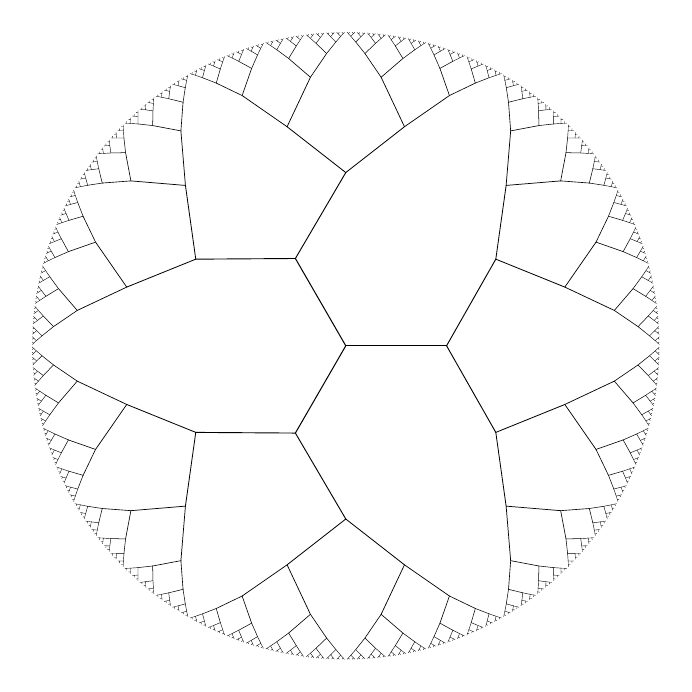
\begin{tikzpicture}[
  x=\ArbolTresRegularEscala,y=\ArbolTresRegularEscala,
  draw=black,line cap=round,line join=round]
  \path[use as bounding box] (-1.01,-1.01) rectangle (1.01,1.01);
  % Argumentos: nivel, angulo central, semiancho del sector, x e y del padre.
  \def\arboltresrama#1#2#3#4#5{%
    \begingroup
    \ifnum#1=1\relax
      \def\arboltresradio{.32}%
    \else\ifnum#1=2\relax
      \def\arboltresradio{.55}%
    \else
      \pgfmathsetmacro{\arboltresradio}{1-.28*pow(.5,#1-3)}%
    \fi\fi
    \pgfmathsetmacro{\arboltresx}{\arboltresradio*cos(#2)}%
    \pgfmathsetmacro{\arboltresy}{\arboltresradio*sin(#2)}%
    \pgfmathsetmacro{\arboltresgrosor}{max(.12,.4-.035*#1)}%
    \draw[line width=\arboltresgrosor pt] (#4,#5)--(\arboltresx,\arboltresy);
    \ifnum#1<\ArbolTresRegularNiveles\relax
      \pgfmathtruncatemacro{\arboltresnivel}{#1+1}%
      \pgfmathsetmacro{\arboltressector}{#3/2}%
      \foreach \arboltressigno in {-1,1}{%
        \pgfmathsetmacro{\arboltresangulo}{#2+\arboltressigno*\arboltressector}%
        \edef\arboltresllamada{\noexpand\arboltresrama
          {\arboltresnivel}{\arboltresangulo}{\arboltressector}{\arboltresx}{\arboltresy}}%
        \arboltresllamada
      }%
    \else
      % Cada extremo continua ramificandose indefinidamente.
      \pgfmathsetmacro{\arboltresfinal}{1-.28*pow(.5,#1-2)}%
      \foreach \arboltressigno in {-1,1}{%
        \pgfmathsetmacro{\arboltresangulo}{#2+\arboltressigno*#3/2}%
        \draw[line width=.12pt]
          (\arboltresx,\arboltresy)--(\arboltresangulo:\arboltresfinal);
      }%
    \fi
    \endgroup
  }
  \arboltresrama{1}{0}{60}{0}{0}
  \arboltresrama{1}{120}{60}{0}{0}
  \arboltresrama{1}{240}{60}{0}{0}
\end{tikzpicture}
\endgroup

% Opcional, antes de \input: \def\ArbolTresRegularNiveles{8}
%                           \def\ArbolTresRegularEscala{4cm}
% La raiz tiene tres hijos a 120 grados; los demas vertices tienen dos hijos.
% Las bifurcaciones de la periferia representan la continuacion infinita.
% No se dibuja una circunferencia de cierre, que introduciria ciclos.
\begingroup
\providecommand{\ArbolTresRegularNiveles}{8}
\providecommand{\ArbolTresRegularEscala}{4cm}
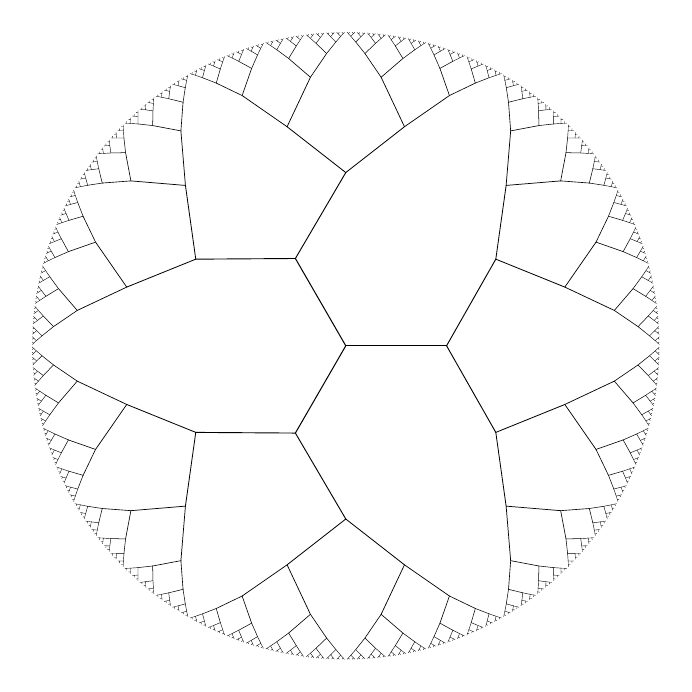
\begin{tikzpicture}[
  x=\ArbolTresRegularEscala,y=\ArbolTresRegularEscala,
  draw=black,line cap=round,line join=round]
  \path[use as bounding box] (-1.01,-1.01) rectangle (1.01,1.01);
  % Argumentos: nivel, angulo central, semiancho del sector, x e y del padre.
  \def\arboltresrama#1#2#3#4#5{%
    \begingroup
    \ifnum#1=1\relax
      \def\arboltresradio{.32}%
    \else\ifnum#1=2\relax
      \def\arboltresradio{.55}%
    \else
      \pgfmathsetmacro{\arboltresradio}{1-.28*pow(.5,#1-3)}%
    \fi\fi
    \pgfmathsetmacro{\arboltresx}{\arboltresradio*cos(#2)}%
    \pgfmathsetmacro{\arboltresy}{\arboltresradio*sin(#2)}%
    \pgfmathsetmacro{\arboltresgrosor}{max(.12,.4-.035*#1)}%
    \draw[line width=\arboltresgrosor pt] (#4,#5)--(\arboltresx,\arboltresy);
    \ifnum#1<\ArbolTresRegularNiveles\relax
      \pgfmathtruncatemacro{\arboltresnivel}{#1+1}%
      \pgfmathsetmacro{\arboltressector}{#3/2}%
      \foreach \arboltressigno in {-1,1}{%
        \pgfmathsetmacro{\arboltresangulo}{#2+\arboltressigno*\arboltressector}%
        \edef\arboltresllamada{\noexpand\arboltresrama
          {\arboltresnivel}{\arboltresangulo}{\arboltressector}{\arboltresx}{\arboltresy}}%
        \arboltresllamada
      }%
    \else
      % Cada extremo continua ramificandose indefinidamente.
      \pgfmathsetmacro{\arboltresfinal}{1-.28*pow(.5,#1-2)}%
      \foreach \arboltressigno in {-1,1}{%
        \pgfmathsetmacro{\arboltresangulo}{#2+\arboltressigno*#3/2}%
        \draw[line width=.12pt]
          (\arboltresx,\arboltresy)--(\arboltresangulo:\arboltresfinal);
      }%
    \fi
    \endgroup
  }
  \arboltresrama{1}{0}{60}{0}{0}
  \arboltresrama{1}{120}{60}{0}{0}
  \arboltresrama{1}{240}{60}{0}{0}
\end{tikzpicture}
\endgroup

% Opcional, antes de \input: \def\ArbolTresRegularNiveles{8}
%                           \def\ArbolTresRegularEscala{4cm}
% La raiz tiene tres hijos a 120 grados; los demas vertices tienen dos hijos.
% Las bifurcaciones de la periferia representan la continuacion infinita.
% No se dibuja una circunferencia de cierre, que introduciria ciclos.
\begingroup
\providecommand{\ArbolTresRegularNiveles}{8}
\providecommand{\ArbolTresRegularEscala}{4cm}
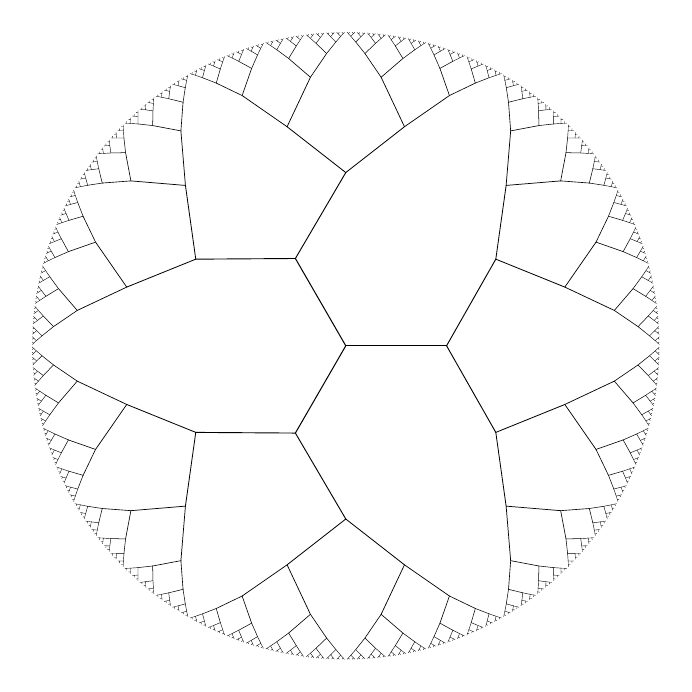
\begin{tikzpicture}[
  x=\ArbolTresRegularEscala,y=\ArbolTresRegularEscala,
  draw=black,line cap=round,line join=round]
  \path[use as bounding box] (-1.01,-1.01) rectangle (1.01,1.01);
  % Argumentos: nivel, angulo central, semiancho del sector, x e y del padre.
  \def\arboltresrama#1#2#3#4#5{%
    \begingroup
    \ifnum#1=1\relax
      \def\arboltresradio{.32}%
    \else\ifnum#1=2\relax
      \def\arboltresradio{.55}%
    \else
      \pgfmathsetmacro{\arboltresradio}{1-.28*pow(.5,#1-3)}%
    \fi\fi
    \pgfmathsetmacro{\arboltresx}{\arboltresradio*cos(#2)}%
    \pgfmathsetmacro{\arboltresy}{\arboltresradio*sin(#2)}%
    \pgfmathsetmacro{\arboltresgrosor}{max(.12,.4-.035*#1)}%
    \draw[line width=\arboltresgrosor pt] (#4,#5)--(\arboltresx,\arboltresy);
    \ifnum#1<\ArbolTresRegularNiveles\relax
      \pgfmathtruncatemacro{\arboltresnivel}{#1+1}%
      \pgfmathsetmacro{\arboltressector}{#3/2}%
      \foreach \arboltressigno in {-1,1}{%
        \pgfmathsetmacro{\arboltresangulo}{#2+\arboltressigno*\arboltressector}%
        \edef\arboltresllamada{\noexpand\arboltresrama
          {\arboltresnivel}{\arboltresangulo}{\arboltressector}{\arboltresx}{\arboltresy}}%
        \arboltresllamada
      }%
    \else
      % Cada extremo continua ramificandose indefinidamente.
      \pgfmathsetmacro{\arboltresfinal}{1-.28*pow(.5,#1-2)}%
      \foreach \arboltressigno in {-1,1}{%
        \pgfmathsetmacro{\arboltresangulo}{#2+\arboltressigno*#3/2}%
        \draw[line width=.12pt]
          (\arboltresx,\arboltresy)--(\arboltresangulo:\arboltresfinal);
      }%
    \fi
    \endgroup
  }
  \arboltresrama{1}{0}{60}{0}{0}
  \arboltresrama{1}{120}{60}{0}{0}
  \arboltresrama{1}{240}{60}{0}{0}
\end{tikzpicture}
\endgroup

% Opcional, antes de \input: \def\ArbolTresRegularNiveles{8}
%                           \def\ArbolTresRegularEscala{4cm}
% La raiz tiene tres hijos a 120 grados; los demas vertices tienen dos hijos.
% Las bifurcaciones de la periferia representan la continuacion infinita.
% No se dibuja una circunferencia de cierre, que introduciria ciclos.
\begingroup
\providecommand{\ArbolTresRegularNiveles}{8}
\providecommand{\ArbolTresRegularEscala}{4cm}
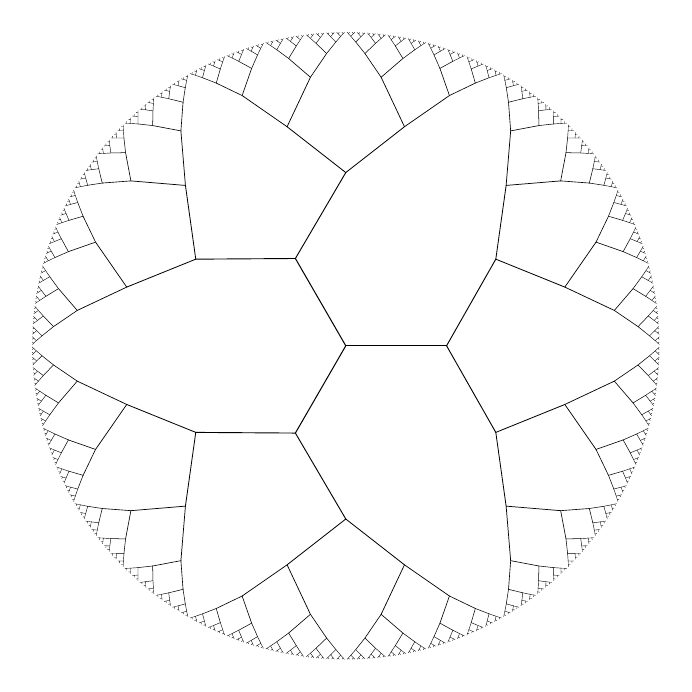
\begin{tikzpicture}[
  x=\ArbolTresRegularEscala,y=\ArbolTresRegularEscala,
  draw=black,line cap=round,line join=round]
  \path[use as bounding box] (-1.01,-1.01) rectangle (1.01,1.01);
  % Argumentos: nivel, angulo central, semiancho del sector, x e y del padre.
  \def\arboltresrama#1#2#3#4#5{%
    \begingroup
    \ifnum#1=1\relax
      \def\arboltresradio{.32}%
    \else\ifnum#1=2\relax
      \def\arboltresradio{.55}%
    \else
      \pgfmathsetmacro{\arboltresradio}{1-.28*pow(.5,#1-3)}%
    \fi\fi
    \pgfmathsetmacro{\arboltresx}{\arboltresradio*cos(#2)}%
    \pgfmathsetmacro{\arboltresy}{\arboltresradio*sin(#2)}%
    \pgfmathsetmacro{\arboltresgrosor}{max(.12,.4-.035*#1)}%
    \draw[line width=\arboltresgrosor pt] (#4,#5)--(\arboltresx,\arboltresy);
    \ifnum#1<\ArbolTresRegularNiveles\relax
      \pgfmathtruncatemacro{\arboltresnivel}{#1+1}%
      \pgfmathsetmacro{\arboltressector}{#3/2}%
      \foreach \arboltressigno in {-1,1}{%
        \pgfmathsetmacro{\arboltresangulo}{#2+\arboltressigno*\arboltressector}%
        \edef\arboltresllamada{\noexpand\arboltresrama
          {\arboltresnivel}{\arboltresangulo}{\arboltressector}{\arboltresx}{\arboltresy}}%
        \arboltresllamada
      }%
    \else
      % Cada extremo continua ramificandose indefinidamente.
      \pgfmathsetmacro{\arboltresfinal}{1-.28*pow(.5,#1-2)}%
      \foreach \arboltressigno in {-1,1}{%
        \pgfmathsetmacro{\arboltresangulo}{#2+\arboltressigno*#3/2}%
        \draw[line width=.12pt]
          (\arboltresx,\arboltresy)--(\arboltresangulo:\arboltresfinal);
      }%
    \fi
    \endgroup
  }
  \arboltresrama{1}{0}{60}{0}{0}
  \arboltresrama{1}{120}{60}{0}{0}
  \arboltresrama{1}{240}{60}{0}{0}
\end{tikzpicture}
\endgroup
